\documentclass[10pt]{article}\usepackage[nu,correction]{esial}
\CSH\sloppy
\usepackage[utf8]{inputenc}
\usepackage{url}
\usepackage{geometry}
\usepackage{fancybox,moreverb}

\newcommand{\cd}[1]{\medskip\noindent\file{\null\hspace{-1em}[#1] }}
\newcommand{\touche}[1]{\hbox{$<$#1$>$}}
\newcommand{\ctrl}[1]{\touche{ctrl-#1}}
\newcommand{\tab}{\touche{TAB}}
%\hypersetup{colorlinks=false,pdfborder={0 0 0}}

\begin{document}
\title{TD2: Encore des pointeurs\ldots}
\maketitle

\bigskip\bigskip\Exercice Un programme C contient la déclaration suivante\,:

\medskip

\begin{boxedverbatim}
  char *couleur[6] = {"rouge", "vert", "bleu", "blanc", "noir", "jaune"};

  char **pcoul = couleur;
\end{boxedverbatim}

\Question Que représente {\tt couleur}? Et \texttt{pcoul}?

\begin{Reponse}
  C'est un tableau de 6 pointeurs vers des chaines de caractères. 

  Du moins, c'est l'explication classique, mais en fait pas tout à
  fait. J'ai dit en amphi que la différence entre \verb+char*+ et
  \verb+char[]+ est l'une des choses les plus obscures du langage C,
  l'une des seules choses qui file des remords aux concepteurs. 

  \textbf{La vérité, c'est que le standard dit que quand on utilise un
    tableau dans une expression, il se fait passer pour un pointeur
    vers la première case du tableau} (sauf en argument de
  \verb+sizeof()+, de \verb+&+ ou quand c'est une chaine de caractères
  pour initialiser un pointeur). Cette page l'explique très bien:
  \url{http://openclassrooms.com/courses/la-verite-sur-les-tableaux-et-pointeurs-en-c}

  Donc, couleur est bien un tableau de pointeurs comme sur le schéma
  ci-dessous, mais quand on utilise couleur dans une expression, il se
  fait passer pour l'adresse de sa première case.  C'est assez
  différent de \texttt{pcoul}, qui lui est un pointeur, un vrai. C'est
  donc un bout de mémoire où est écrit une adresse.

  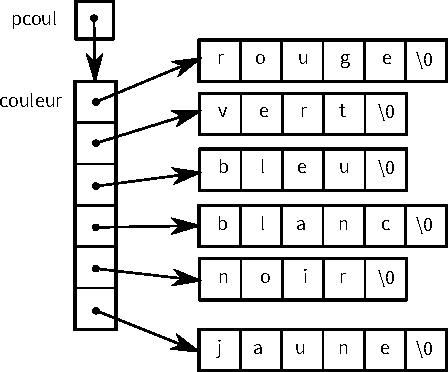
\includegraphics{memoire-couleur.pdf}

  Si on se sent l'humeur taquine, on peut faire remarquer qu'il est
  probable que les différentes chaines de caractères soient
  consécutives en mémoire. Cela donne le schéma suivant: \\

  \noindent
  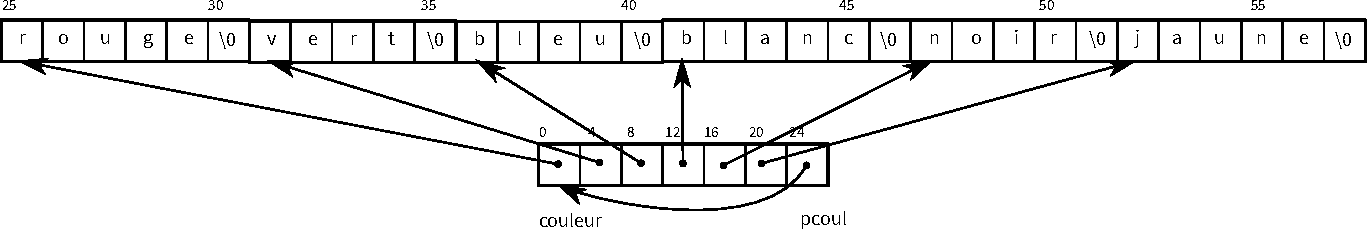
\includegraphics[width=\linewidth]{memoire-couleur2.pdf}

  J'ai séparé les chaines de caractère litérales des tableaux car dans
  l'espace d'adressage du processus, les chaines vont être dans les
  globales constantes (avec le code), et les variables vont être dans
  les globales modifiables si ce sont des globales, ou dans la pile si
  ce sont des variables locales. A vous de voir si vous voulez dire
  l'entière vérité ou pas.
\end{Reponse}

\Question Que  désigne {\tt couleur + 2}?

\begin{Reponse}
  C'est l'adresse de la seconde case du tableau, c'est-à-dire
  \verb|&(couleur[2])|
\end{Reponse}

\Question Quelle est la valeur de {\tt *couleur}?

\begin{Reponse}
  C'est \verb|couleur[0]|, c'est à dire l'adresse de la chaîne
  \texttt{"rouge"}, qui se trouve quelque part dans le segment data du
  processus (là où il y a le code et les globales).
\end{Reponse}

\Question Quelle est la valeur de {\tt *couleur + 2}\,?

\begin{Reponse}
\begin{verbatim} 
    couleur + 2 = &couleur[2] et *(couleur+2)=couleur[2]="bleu"
    *couleur = couleur[0] = "rouge"
    *couleur+2 = "uge"
\end{verbatim}

\noindent\verb?*couleur? pointe sur le premier élément de la chaine ``rouge''
soit 'r'. Si on rajoute 2, on décale de deux cases, et ça pointera sur
'u'. La fin de la chaine est après 'e' de "rouge".
\end{Reponse}

\Question Quelle est la valeur de {\tt *(*(couleur + 5) +3)}\,? (Même
question avec +4, +5, +6).

\begin{Reponse}
\begin{verbatim} 
   *(*(couleur + 5) +3) = 'n' 
   En effet : 
     *(couleur + 5) = "jaune" , "jaune" étant situé à couleur[5] 
     *(couleur + 5) +3 = "ne"

   *(*(couleur + 5) +4) = 'e' 
   *(*(couleur + 5) +5) = '\0' 
   *(*(couleur + 5) +6) = 'c' , c quelconque 
\end{verbatim}
~
\end{Reponse}




\bigskip\bigskip\Exercice {\bf Pointeurs et structures.}
%----------------------------------------

Soit le type suivant:


\medskip

\begin{boxedverbatim}
  typedef struct {
    char nom[MAX_CAR];
    int  rayon;  
  } planete_t;
\end{boxedverbatim}


\Question Écrire un constructeur pour ce type \texttt{planete\_t}.

\begin{Reponse}
  \begin{boxedverbatim} 
planete_t *planete_create(char *nom, int rayon) {
    planete\_t *p1;
    p1 = (planete_t *) malloc (sizeof(planete_t));
    strcpy(p1->nom, nom);
    p1->rayon = rayon;
    return p1;
}  \end{boxedverbatim}
~
\end{Reponse}
	  
\Question Écrire une fonction qui saisit les données relatives à une
planète, et crée une planète en conséquence.

\begin{Reponse}
  \begin{boxedverbatim} 
planete_t *planete_saisir(){
  char nom[32];
  int rayon;

  printf("Donner nom planète : ");
  scanf ("%s",nom);
  printf("Donner son rayon : ");
  scanf ("%d",&rayon);
  return planete_create(nom,rayon);
}  \end{boxedverbatim}
~
\end{Reponse}

\Question Écrire une fonction qui duplique une planète (un
\textit{copy constructor}). 

\begin{Reponse}
  \noindent
  \begin{boxedverbatim} 
// Version compliquée

planete_t* planete_dup(planete_t *p){

  planete_t *res;
  res=(planete_t*)
      malloc(sizeof(planete_t));
  
  strcpy(res->nom, p->nom);
  p1->rayon = p->rayon;
  
  return p1;
} \end{boxedverbatim}
~~~
  \begin{boxedverbatim} 
// Version simple

planete_t* planete_dup(planete_t *p){

  return planete_create(p->nom, 
                        p->rayon);
} 






\end{boxedverbatim}
~
\end{Reponse}

\Question  Soit l'extrait suivant permettant de tester les fonctions
précédentes;


\medskip


\begin{boxedverbatim}
void main() {

  planete_t p;
  planete_t *ptr_p;
  ptr_p = planete_saisir();
  p = *ptr_p;
  printf("%s %d \n", p.nom, p.rayon);
  ptr_p = planete_dup(p);
  printf("%s %d \n", ptr_p->nom, ptr_p->rayon);
}
\end{boxedverbatim}


\bigskip Comment s'analysent les types des différentes références
suivantes\,:

\bigskip

\begin{tabular}{|p{.2\linewidth}|p{.3\linewidth}|}
  \hline
  Référence          &   Type  \\\hline
  \verb+ptr_p+       &         \\\hline                  
  \verb+*ptr_p+      &         \\\hline            
  \verb+ptr_p->nom+  &         \\\hline
  \verb+ptr_p->rayon+&         \\\hline
  \verb+p+           &         \\\hline
  \verb+&p+          &         \\\hline
  \verb+p.nom+       &         \\\hline
  \verb+p.rayon+     &         \\\hline
\end{tabular}


\begin{Reponse}

\begin{tabular}{|p{.2\linewidth}|p{.3\linewidth}|}
  \hline
  Référence          &          Type         \\\hline
  \verb+ptr_p+       &  \verb+planete_t *+         \\\hline                  
  \verb+*ptr_p+      &  \verb+planete_t+           \\\hline            
  \verb+ptr_p->nom+  &  \verb+char []+\\\hline
  \verb+ptr_p->rayon+& int\\\hline
  \verb+p+           & \verb+planete_t+\\\hline
  \verb+&p+          & \verb+planete_t*+\\\hline
  \verb+p.nom+       & \verb+char []+\\\hline
  \verb+p.rayon+     & \verb+int+\\\hline
\end{tabular}
~
\end{Reponse}


 

\newpage
\bigskip\bigskip\Exercice {\bf Chaînes de caractères.}
%--------------------------------------

\Question
Écrire une fonction {\tt PremierCar(\ldots)} qui renvoie l'adresse de
la première occurence du 
caractère {\tt c} dans une chaîne de caractères dont l'adresse (du
premier caractère) est passé à l'argument {\tt ptrCar}\,:

\run{char *PremierCar(char c, char *ptrCar)}

\Question
Écrire la fonction {\tt int main(int argc, char *argv[ ])} permettant
de tester la fonction. Voici un exemple d'exécution:

\medskip

\begin{boxedverbatim}
$ ./occurence o Bonjour
La premiere occurence de 'o' dans 'Bonjour' est en position 1
$ ./occurence z Bonjour
'z' n'est pas dans Bonjour.
\end{boxedverbatim}

\begin{Reponse}
  Cet exercice a été déjà fait en TP2 mais il y a une différence dans
  le type de retour qui est un pointeur au lieu d'un entier. Aussi, on
  fait usage des arguments en ligne de commande.

\begin{boxedverbatim}
#include <stdio.h>

char *PremierCar(char c, char *ptrCar){
  do {
    if (*ptrCar == c)
      return ptrCar;
  } while (*(ptrCar++));

  return NULL;
}

int main(int argc, char * argv[]){

  char c, *str, *adrPremCar;

  c = argv[1][0]; // argv[1] étant un pointeur vers une chaine de car.
                  // argv[1][0] est le premier car de cette chaine
  str = argv[2];
  adrPremCar = PremierCar(c,str);

  if (adrPremCar == NULL) 
    printf ("'%c' n'est pas dans %s.\n",c,str);
  else
    printf ("La premiere occurence de '%c' dans %s est en position %d.\n",
            c, str, adrPremCar - str);
}
\end{boxedverbatim}
\end{Reponse}
    



\bigskip\bigskip\Exercice {\bf Filiation.}
%--------------------------------

Sous Unix, il existe un ensemble de pointeurs représentant la
filiation des  processus. 
%
Dans la figure~\ref{filiation}, {\tt fils A} est le premier processus
fils créé par le processus père, {\tt fils B} est le deuxième fils
créé par le processus père \ldots etc.
Chaque fils peut évidemment créer des fils, et le père est également le
fils d'un autre processus.
%
Chaque processus est caractérisé par un numéro (un entier positif).

\bigskip\bigskip
\begin{figure}[h]
  \centerline{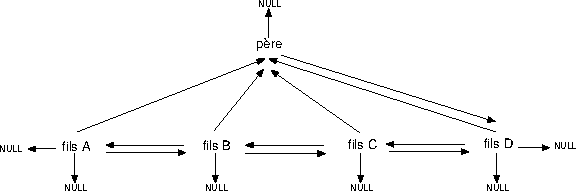
\includegraphics[width=\linewidth]{filiation.pdf}}
  \caption[]
	  {{\it Filiation sous Unix}}
	  \label{filiation}
\end{figure}
\bigskip

\Question Représenter schématiquement, sous la forme d'une structure
de données, un n\oe ud (c'est à dire un processus) de cette filiation,
puis écrire la définition de cette structure en C.

\Question Le processus repéré par la variable pointeur {\tt p} vient
de créer un processus fils de numéro {\tt no}.  Écrire en C la
fonction {\tt maj} qui met à jour la filiation des processus.

\begin{Reponse}
\vspace{-.7cm}
\begin{verbatim}


typedef struct proc {
  unsigned int noproc;
  struct proc *pere, *frere_g, *frere_d, *dernier_fils;
} proc_t;

void maj(proc_t *p, int no){
  proc_t *fils;
  fils = (proc_t *) malloc (sizeof(proc_t));

  fils->noproc = no;
  fils->pere = p;
  fils->frere_d = NULL;
  fils->dernier_fils = NULL 

  if (p->dernier_fils != NULL){
    //le père a déjà des fils, le dernier fils devient le frère à
    //gauche et aura un frère à sa droite
    fils->frere_g = p->dernier_fils;
    p->dernier_fils->frere_d = fils;
  } else {// le père n'avait pas de fils
    fils->frere_g = NULL;
    p->dernier_fils = fils;
  } 
}
\end{verbatim}
~
\end{Reponse}



\end{document}

%%% Local Variables:
%%% coding: utf-8
